\subsection{Skalrum}

\newcounter{lppauses}

\begin{frame}
\frametitle{Skalrum}

\begin{columns}[c]

\column{.5\textwidth}

\begin{itemize}[<+(1)->]
\item Vattnet modelleras som en höjdkarta: $h(\vec{x})$
\item Laplacian Pyramid
\setcounter{lppauses}{\thebeamerpauses}
    \begin{itemize}[<+(1)->]
    \item Olika våglängder sparas på olika griddar
    \item T.ex. \mbox{1--2 m}, \mbox{2--4 m}, \mbox{4--8 m}, \mbox{8--16 m}, o.s.v.
    \item Gridupplösningen avgörs av kortaste våglängden
    \end{itemize}
\item Vågekvationen löses separat på varje grid\\
$\left(\displaystyle \frac{\partial^2 h}{\partial t^2} = c^2\nabla^2h\right)$
\item Höjdkartan ges av summan av alla griddar
\item Geometrisk summa $\Rightarrow O(n)$
\end{itemize}

\column{.5\textwidth}

\uncover<\thelppauses->{
\begin{figure}
\centering
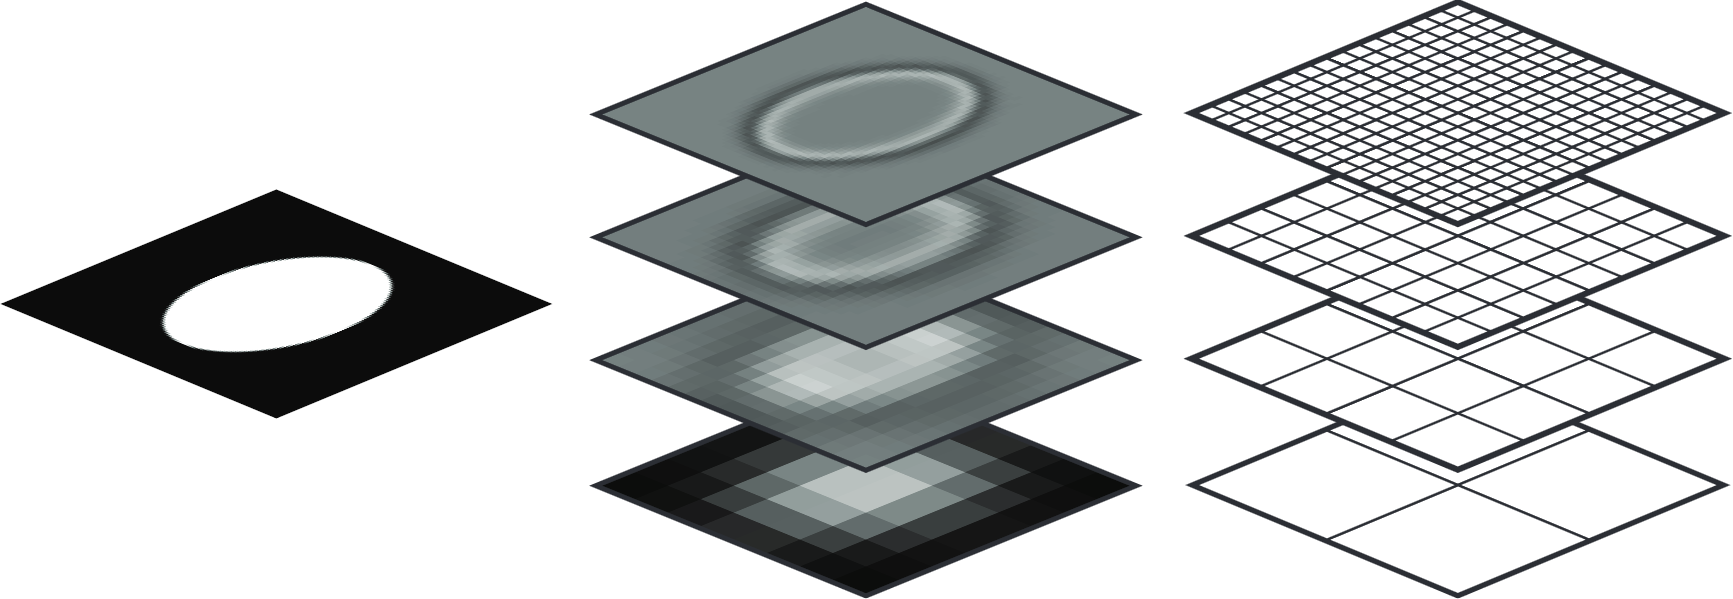
\includegraphics[width=\textwidth]{Images/Other/LPD}
\end{figure}
}

\end{columns}

\end{frame}